\begin{merkbox}[Merke: Zufallsexperiment]
Ein \textbf{Zufallsexperiment} liegt vor, wenn alle vier Bedingungen erfüllt sind:
\begin{enumerate}[label=\arabic*.]
    \item Es gibt mindestens zwei mögliche Ergebnisse.
    \item Alle möglichen Ergebnisse sind vorher bekannt.
    \item Welches Ergebnis eintritt, kann man nicht vorhersagen.
    \item Das Experiment lässt sich (zumindest gedanklich) beliebig oft unter gleichen Bedingungen wiederholen.
\end{enumerate}
Die Menge aller möglichen Ergebnisse heißt \textbf{Ergebnisraum} $\Omega$ (sprich: Omega).\\
Beispiel Würfelwurf: $\Omega = \{1;\,2;\,3;\,4;\,5;\,6\}$.
\end{merkbox}

\begin{merkbox}[Merke: Baumdiagramm]
Ein \textbf{Baumdiagramm} zeigt alle Ergebnisse übersichtlich. Jede Stufe des Experiments bekommt eine eigene Ebene, jedes mögliche Teilergebnis einen eigenen Ast. Jeder Weg vom Start bis zum Ende (ein \textbf{Pfad}) ergibt genau ein Ergebnis.
\end{merkbox}

\begin{beispielbox}[Beispiel: Münze zweimal werfen]
Eine Münze wird zweimal geworfen. W bedeutet Wappen, Z bedeutet Zahl.
\begin{center}
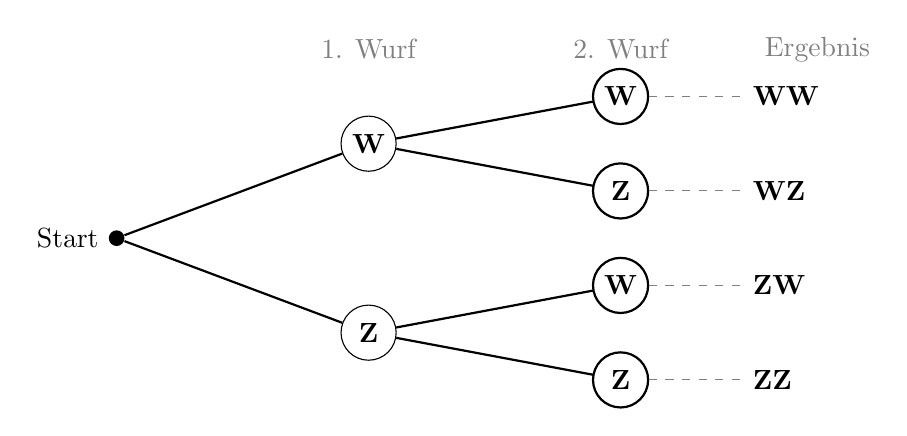
\begin{tikzpicture}[
    grow=right,
    level distance=3.2cm,
    level 1/.style={sibling distance=2.4cm},
    level 2/.style={sibling distance=1.2cm},
    knoten/.style={circle, draw, minimum size=7mm, inner sep=0pt, font=\bfseries},
    edge from parent/.style={draw, thick}
]
\node[fill, circle, inner sep=2pt, label=left:Start] {}
    child {node[knoten] {Z}
        child {node[knoten] (zz) {Z}}
        child {node[knoten] (zw) {W}}
    }
    child {node[knoten] {W}
        child {node[knoten] (wz) {Z}}
        child {node[knoten] (ww) {W}}
    };
\foreach \n/\t in {ww/WW, wz/WZ, zw/ZW, zz/ZZ} {
    \draw[dashed, gray] (\n.east) -- ++(1.2cm,0) node[right, black] {\textbf{\t}};
}
\node[gray] at (3.2, 2.4) {1. Wurf};
\node[gray] at (6.4, 2.4) {2. Wurf};
\node[gray] at (8.9, 2.4) {Ergebnis};
\end{tikzpicture}
\end{center}
$\Omega = \{\text{WW};\,\text{WZ};\,\text{ZW};\,\text{ZZ}\}$, also 4 Ergebnisse.
\end{beispielbox}
